\documentclass[conference]{IEEEtran}
% \IEEEoverridecommandlockouts
% The preceding line is only needed to identify funding in the first footnote. If that is unneeded, please comment it out.
\usepackage{cite}
\usepackage{amsmath,amssymb,amsfonts}
\usepackage{algorithmic}
\usepackage{graphicx, float}
\usepackage{textcomp}
\usepackage{xcolor}
\usepackage{url}
\def\BibTeX{{\rm B\kern-.05em{\sc i\kern-.025em b}\kern-.08em
    T\kern-.1667em\lower.7ex\hbox{E}\kern-.125emX}}
\def\code#1{\texttt{#1}}
\begin{document}

\title{Room Optimisation Algorithm\\
{\footnotesize Digital Signal Processing May Assignment}
\thanks{Identify applicable funding agency here. If none, delete this.}
}

\author{\IEEEauthorblockN{1\textsuperscript{st} Alex Booth}
\IEEEauthorblockA{\textit{School of Computing, Science and Engineering} \\
\textit{The University of Salford}}}

\maketitle

\begin{abstract}
    This report describes a successful attempt to create a basic room compensation filter in MATLAB.
    The compensation filter is created by using fourier analysis to deduce a room's frequency response.
    The methodology is described in detail, and the code used to create the compensation filter is appended in an appendix.
    The results are presented in figures, which are analysed and discussed.

\end{abstract}cccc

\section{Introduction}
    The compensation of a room's coloration of an acoustic signal has many applications.
    In the context of loudspeaker development, compensating for the response of a room allows the loudspeaker to theoretically function identically, no matter the room it is placed in.
    Algorithms to compensate for the frequency and phase issues caused by rooms are built into many commercial loudspeakers, and room correction is fast becoming a mainstay of professional recording studios.


\section{Theory}
    \subsection{Impulse Responses}
        To compensate for the frequency response of a room so that a listener in the room hears the output of a loudspeaker without any coloration of the sound by the room, one must first find and quantify the way the room effects sound produced by the speaker.
        When approaching this task using digital signal processing, finding the room's impulse response allows us to quantify the way it affects any input impulse.
        A digital impulse is a single sample signal with a sample value of 1.
        A more precise mathematical definition is given in Eq.\ref{uSample}:
        \begin{equation}\label{uSample}
            \delta[n] = 
            \begin{cases}
                0, n \neq 0\\
                1, n = 0
            \end{cases}
        \end{equation}
        By knowing the response of a system when the input is an impulse $\delta[n]$, allows the response of the system to any input to be predicted, so long as the system is both linear and shift-invariant \cite{OPPENHEIM}.
        This response to $\delta[n]$ is known as the impulse response, $h[n]$.
        In this digital model, the room's frequency response is effectively a series of filters and so it will be both linear and shift-invariant.
        By convolving $h[n]$ with any input $x[n]$, the output $y[n]$ of the signal flow can be found. 
        The convolution in the digital domain is formulated as a sum, as opposed to the continuous time domain where it is an integral.
        The digital convolution sum is shown in Eq.\ref{conv}
        \newpage
        \begin{equation}\label{conv}
            y[n] = \sum_{k=-\infty}^\infty x[k] h[n-k]
        \end{equation}
        So by computing the convolution sum of an input signal with the impulse response of the room, the output of the room can be found, and thus the effect of the room on the frequency response of a signal.
    \subsection{Test Signals}
        To test the effectiveness of a compensation filter, test signals to be used as input must be devised.
        The frequency and amplitude components of test signals are important, such that the effectiveness of the filter is tested over as wide a range of frequencies and amplitudes as possible.
        Two common input signals used to test digital filters are 'chirps' and 'bursts'.
        A chirp is a pure sine wave signal swept from low to high frequency over it's signal length; it can be swept linearly or logarithmically, and can cover any frequency range as required.
        A linearly swept sine is defined by Eq.\ref{chirp}, where $\phi_0$ is initial phase, $t$ is time, and $f_0$ is initial frequency.
        \begin{equation}\label{chirp}
            x[t] = \sin{[\phi_0 + 2\pi(\frac{c}{2} t^2 + f_0 t)]}
        \end{equation}
        A burst is a short length of pink noise.
        A digital noise signal is non-deterministic and statistically random in it's current sample value, as so it cannot be described to have a frequency or period, as it is almost impossible for it to repeat over a given time period \cite{OPPENHEIM376}.
        This randomness can instead be quantified with a standard deviation $\sigma$, and probability of frequency \& magnitude components arising throughout the signal.
        White noise is the most basic noise signal, with every frequency sharing an equal probability of arising at all times throughout the signal; it has constant power spectral density \cite{CARTER}
        Pink noise, does not have a constant equal probability for any frequency to arise in the signal.
        \begin{figure}[H]
            \centering
            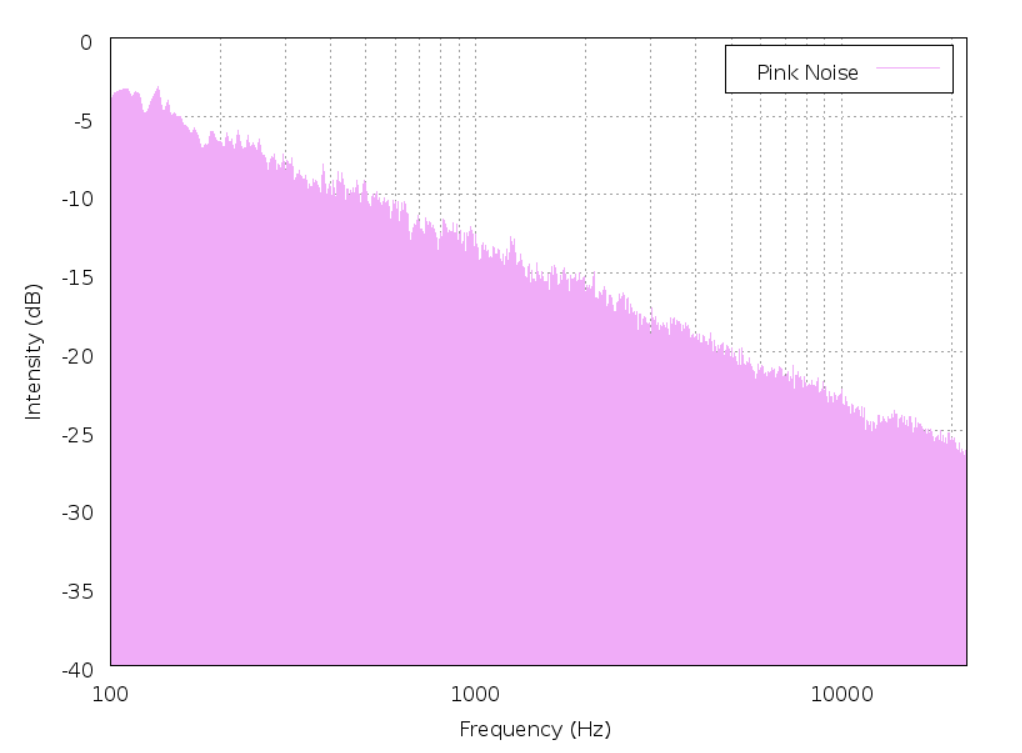
\includegraphics[scale = 0.35]{resources/PinkNoise.png}
            \caption{Frequency Response of Pink Noise \cite{AFIELDS}}
        \end{figure}
        Instead, pink noise's power spectral density is inversely proportional to the frequency of the signal.
        Using pink noise as a test signal is preferred over white noise, as the roll-off in average amplitude over frequency generally follows the equal loudness curve - where the human auditory experience is more sensitive to high frequencies \cite{GENELEC}.
        With white noise the high frequencies naturally dominate the human auditory experience; the frequency roll-off of pink noise compensates for this.
        
    \subsection{Digital Filters}
        In the continuous time audio domain, filters are applied using either passive or active circuits.
        Loudspeakers often use these analog electronic filters to cross-over the optimal frequency pass-bands of a pair of drivers to create an optimum combined system response.
        In the digital, discrete-time domain, filters are realized as linear, shift-invariant systems.
        Digital filters fall into two categories, finite impulse response (FIR) and infinite impulse response (IIR).
        As their names imply, the main difference between the two digital filter types is their impulse responses.
        An IIR filter's  signal flow is recursive and thus - when fed an impulse of $\delta[n]$, the impulse response $h[n]$ is infinitely long.
        An FIR filter has a feed-forward signal flow and so is not recursive and has a finitely long impulse response.
        Equation \ref{FIR} shows the general form of an FIR filter, where the output is equal to the input $x[n]$ convolved with the impulse response of the filter $h[n]$ \cite{JORDAN}:
        \begin{equation}\label{FIR}
            y[n] = \sum_{k=0}^N h_k x_{n-k}
        \end{equation}
        A block diagram for a simple first-order, feed-forward FIR filter is shown in Fig.\ref{BLOCK} \cite{EricTarr2018HAAI}.
        This filter uses a constant time delay, such that as the input frequency increases the phase shift between $x[n]$ and $x[n-1]$ also increases and thus as frequency increases, so does destructive interference.
        \begin{figure}[H]
            \centering
            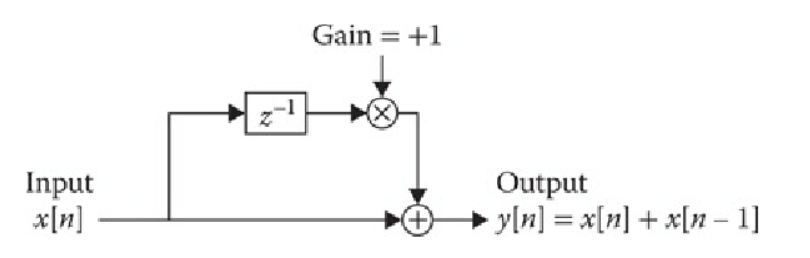
\includegraphics[scale = 0.4]{resources/FIRLPF.png}
            \caption{An FIR low pass filter utilizing a constant time delay}
            \label{BLOCK}
        \end{figure}
        When designing digital filters there are many criteria of performance and description that must be noted.
        For example, whether or not the filter has linear phase response, the order of the filter, the pole and zero plots of the z-transform and the efficiency of the filter.
        An example of a pole-zero plot, obtained after taking the z-transform of a 10th order IIR Butterworth filter, is shown in Fig.\ref{zplot}
        \begin{figure}[H]
            \centering
            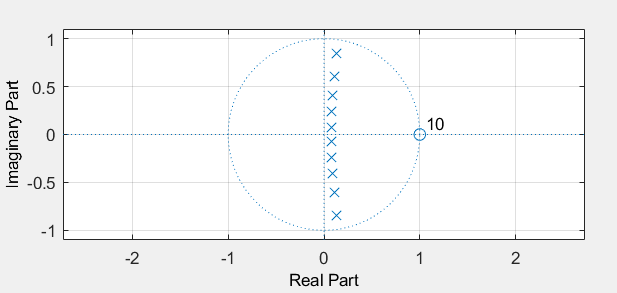
\includegraphics[scale = 0.65]{resources/poleZero.png}
            \caption{Pole-zero plot of a 10th order IIR Butterworth filter}
            \label{zplot}
        \end{figure}
        A pole-zero plot allows various features of a filter to be deduced, for example:
        \begin{itemize}
            \item Stability
            \item Causality
            \item Region of convergence (ROC)
            \item Minimum phase / non minimum phase
        \end{itemize}
        To deduce stability, check to see if all poles are on the left hand side of the plot - if so then the system is stable.

\section{Methodology}
    \subsection{Analyzing the Provided Code}
        A MATLAB script generating an impulse response for a simulated room was provided.
        This section seeks to analyse the methods used to create a simulated room's impulse response
        First, after setting the dimensions of a hypothetical room, the maximum number of room modes in any dimension were calculated with Eq.\ref{eigen}, which defines the eigenfrequencies within a rigid rectangular enclosure \cite{Cox}.
        \begin{equation}\label{eigen}
            f = \frac{c}{2}\sqrt{(\frac{n_x}{L_x})^2+(\frac{n_y}{L_y})^2+(\frac{n_z}{L_z})^2}
        \end{equation}
        A simulated listening point in the room was set, and a for loop was iterated through to calculate the transfer function of the room.
        A 24\textsuperscript{th} order Butterworth FIR filter was then introduced, using the \code{butter()} function to create the filter cleaning any 'impulse response post-ringing'.
        Using the \code{ifft()} function to take an inverse fast fourier transform, the impulse response of the room was found, as exported as the variable $G$.
    
    \subsection{Finding the Room's Frequency Response}
        To determine the effect of a digitally modelled room on a signal given only it's impulse response $h[n]$ (given in the code as $G$), information must first be extracted from the impulse response.
        Given that all test input signals are in the range of $\pm1$, the impulse response is normalized to $\pm1$.
        Next, a fast fourier transform is taken of the impulse response; in MATLAB the \code{fft(a,b)} function returns the fourier transform of $a$ with a resolution of $b$.
        The resolution was set to 1024.
    \subsection{Calculating the Inverse of the Room's Frequency Response}  
        Finding the inverse of the room's frequency response allows a filter that is the complete opposite, and thus will cancel out the effect of the room, to be formulated.
        To find this inverse, the reciprocal of the frequency response from the FFT is taken.
        This gives an equal but opposite frequency response.
        The real part of this inverse is taken (the output of \code{FFT()} is complex), and converted back to an impulse response with the inverse FFT function \code{ifft()}.
        From this impulse response, the frequency and magnitude component of a filter can be extracted from it's impulse response using the \code{freqz()} function.
        Converting the magnitude to dB and plotting against frequency, gives a graph of the frequency response of the inverse filter.
        Using  \code{freqz()}, the frequency response was also taken of the impulse response of the room.
        Both frequency responses were plotted on the same graph, and can be seen in Fig.\ref{origAndInverse1}.
        After confirming from the graph that the filter appeared to be the inverse, the testing phase began.
    \subsection{Formulating and Applying Test Signals}
        A pink noise burst and sine wave chirp were used as test signals.
        To formulate the pink noise as an array of sample values in MATLAB, an object of the \code{dsp.ColoredNoise()} class was created from the DSP toolbox.
        This object takes three arguments upon initialization, the first being the inverse frequency power $\alpha$ of the noise sequence; pink noise's $\alpha = 1$ due it's amplitude being inversely proportional to it's frequency.
        The next two arguments were number of samples per channel, set to 2001, and number of channels, set to 1.
        \begin{figure}[H]
            \centering
            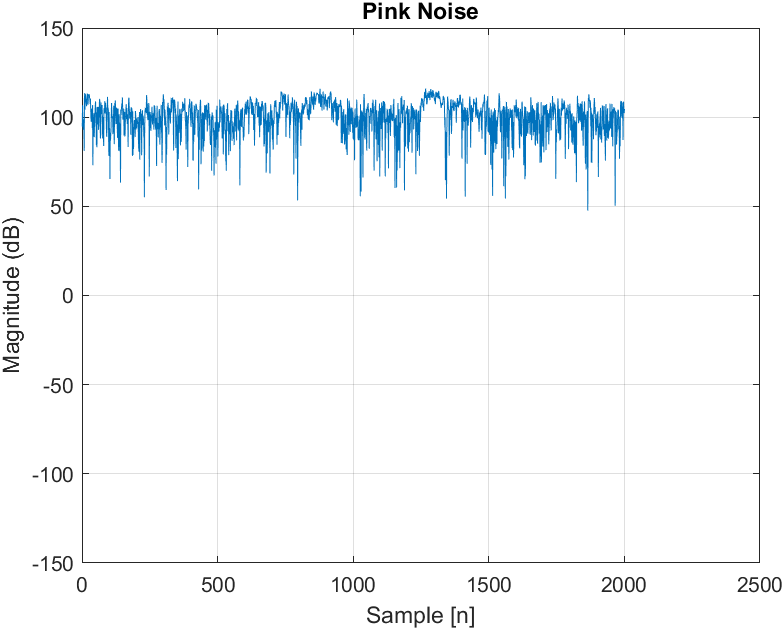
\includegraphics[scale = 0.65]{resources/pinkNoiseGraph.png}
            \caption{Plot of the formulated pink noise test signal}
            \label{pinkNoiseGraph}
        \end{figure}
        To create the sine wave chirp, the \code{chirp()} function was used.
        This function takes an array of sample values as the first argument, initial frequency as the second, and then time for target frequency and target frequency as the third and fourth.
        It was decided to create a chirp that sweeps from 0 to 500Hz, over 2001 samples.
        This gives it the same sample length as the pink noise burst.
        The spectral density of the chirp is shown in Fig.\ref{spectrogram}, where it shows a clear linear sweep of frequency over time:
        \begin{figure}[H]
            \centering
            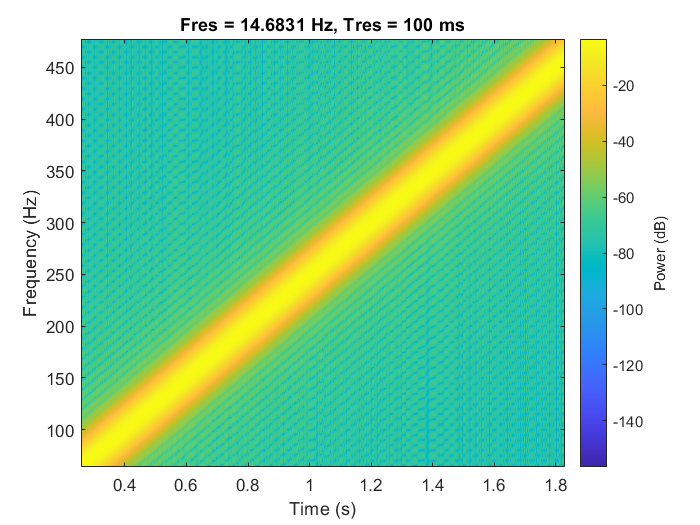
\includegraphics[scale = 0.45]{resources/spectrogram.png}
            \caption{Spectrogram of the chirp}
            \label{spectrogram}
        \end{figure}
        To test the inverse filter, the test signals were first convolved with the impulse response of the room, and then convolved with the impulse response of the compensation filter.
        The two convolutions were converted to decibels and plotted on the same graph, as seen in Figs.\ref{noiseComparison} \& \ref{chirpComparison}.
        As can be seen in Fig.\ref{chirpComparison} distortion is present in the upper frequency band, where it should be flat.
        Revisiting Fig.\ref{origAndInverse1} it can be seen that there are 'ripples' found in the rejection band of the room's frequency response, whilst the inverse filter has a relatively flat pass band and thus doesn't compensate for this distortion.
        Increasing the resolution of the FFT taken of the room's impulse response by twenty times served to eliminate this flat pass band, and allows the inverse filter to compensate for the rejection band 'ripples'.
        The updated graphs of frequency response for the inverse filter and compensated chirp are shown in Figs.\ref{origAndInverse2} \& \ref{chirpComparison2}, respectively.
\section{Results}
    \subsection{Frequency \& Phase Response Figures}
        \begin{figure}[H]
            \centering
            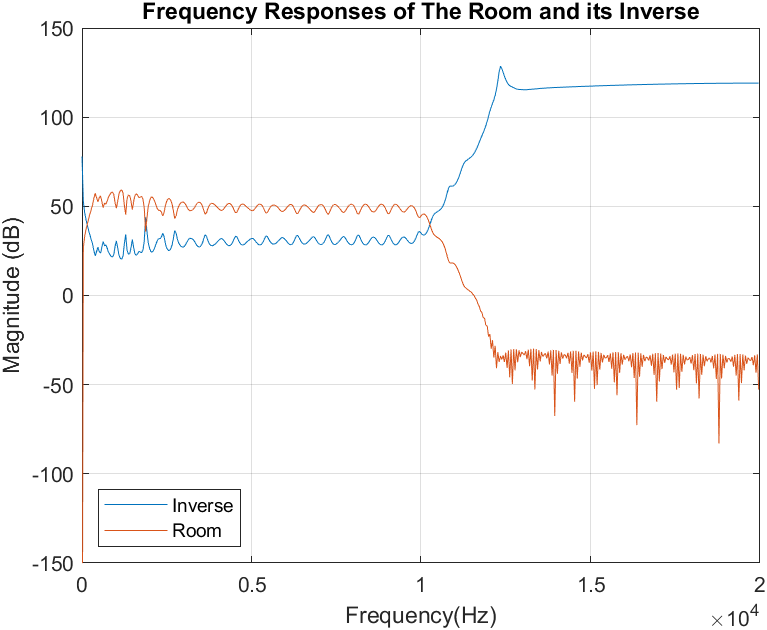
\includegraphics[scale = 0.55]{resources/origAndInverse1.png}
            \caption{Frequency responses of the room and it's inverse filter}
            \label{origAndInverse1}
        \end{figure}
        \begin{figure}[H]
            \centering
            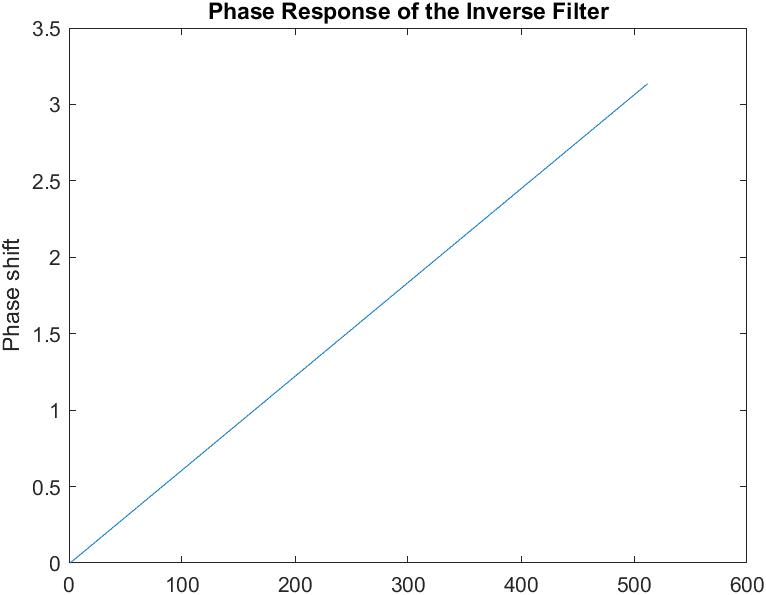
\includegraphics[scale = 0.55]{resources/phaseResp.png}
            \caption{Phase response of the inverse filter}
            \label{phaseResp}
        \end{figure}
        \begin{figure}[H]
            \centering
            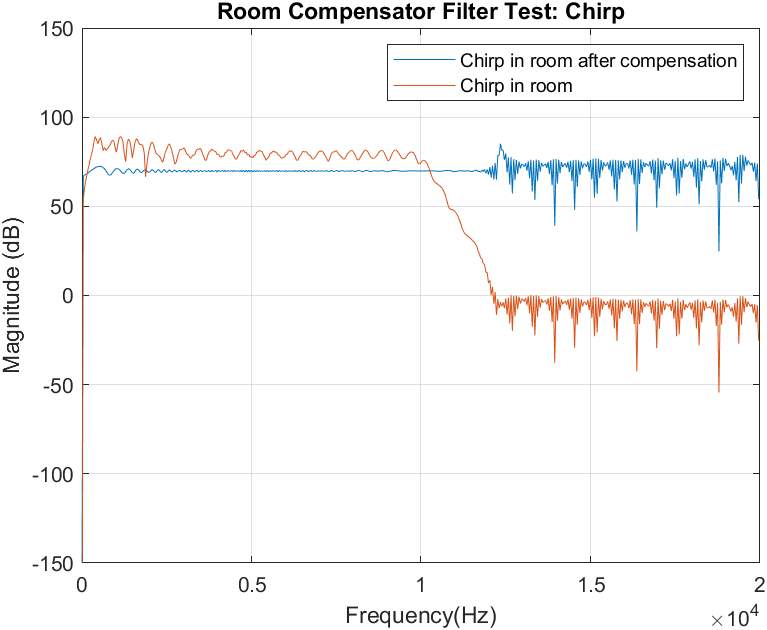
\includegraphics[scale = 0.55]{resources/chirpComparison.png}
            \caption{Frequency responses of the chirp in the room with and without compensation}
            \label{chirpComparison}
        \end{figure}
        \begin{figure}[H]
            \centering
            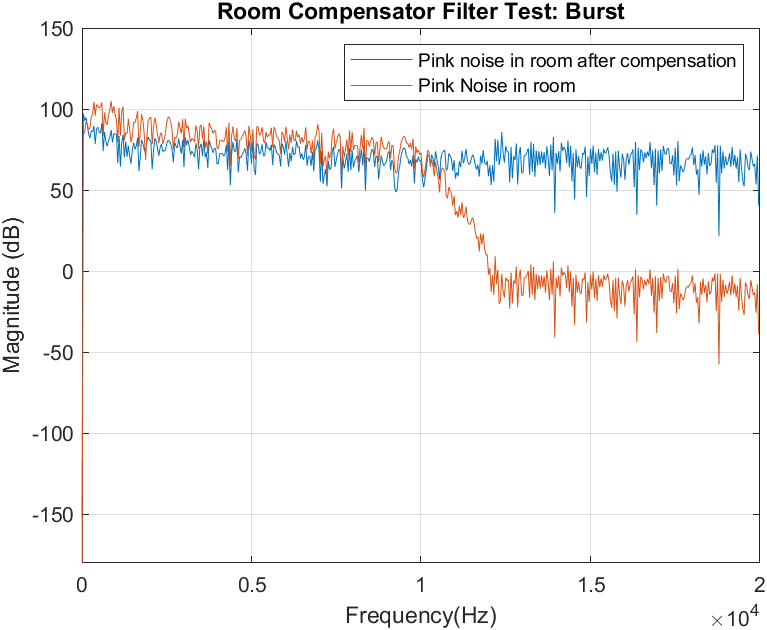
\includegraphics[scale = 0.55]{resources/burstComparison.png}
            \caption{Frequency responses of the burst in the room with and without compensation}
            \label{noiseComparison}
        \end{figure}
        \begin{figure}[H]
            \centering
            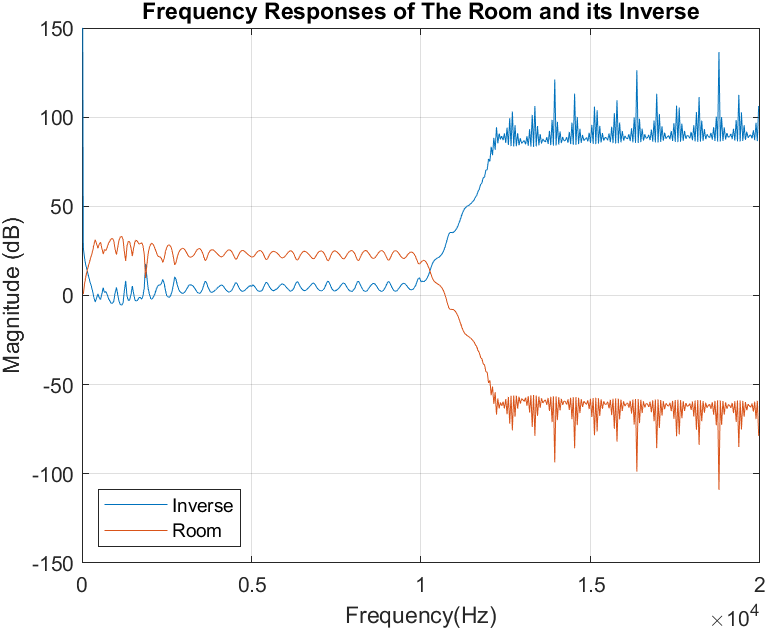
\includegraphics[scale = 0.55]{resources/origAndInverse2.png}
            \caption{Updated frequency responses of the room and it's inverse filter}
            \label{origAndInverse2}
        \end{figure}
        \begin{figure}[H]
            \centering
            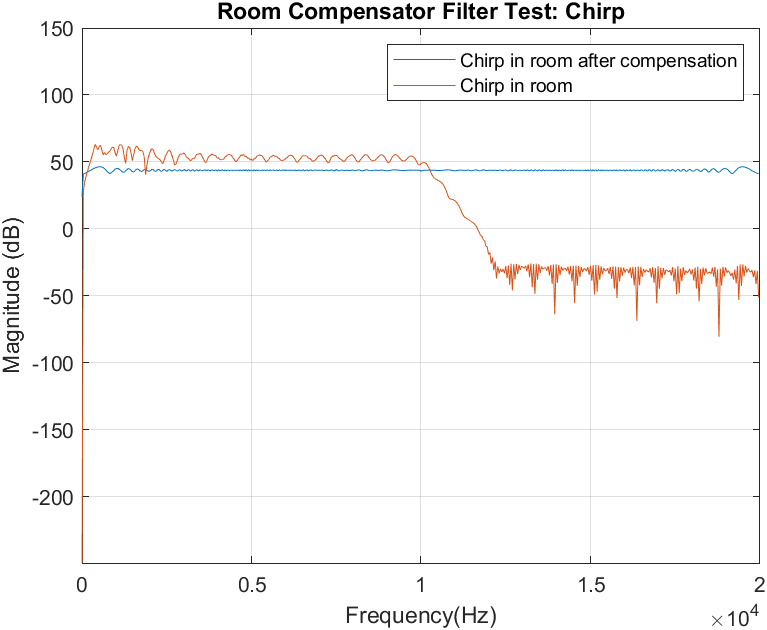
\includegraphics[scale = 0.55]{resources/chirpComparison2.png}
            \caption{Updated frequency responses of the chirp in the room with and without compensation}
            \label{chirpComparison2}
        \end{figure}

\section{Discussion of Results}
    So far in this report, the room and it's impulse response have been treated like a simple filter, being shown as a low-pass filter in Fig.\ref{origAndInverse2}.
    However, upon further inspection of the provided MATLAB script used to generate the impulse response, it can be seen that the low-pass filter has been added in order to 'remove impulse response post ring'.
    As the compensation filter used was not designed using any kind of algorithm or signal flow diagram, but was instead reverse-engineered, it can be assumed that it would be an FIR filter, as it is an inverse of the applied low-pass FIR filter, and has a finitely long impulse response.
    The small 'ripples' found in Fig.\ref{origAndInverse1} can be assumed to be the frequency response of the actual room - as a 10th order Butterworth filter shouldn't have this characteristic.
    The efficiency of the filter designs must also be taken into question.
    As the resolution had to be set to a large number (20480) to compensate for ripples in the frequency response, the comparative time taken to compute the FFT of the impulse response is quite long.
    Investigation into the minimum acceptable resolution that still produces an acceptable inverse filter with no ripples would serve to improve the compensation filter.
    Upon observation of Fig.\ref{phaseResp} it can be seen that the inverse filter has a linear phase response.
    The result is that all frequency components of the input signal to the filter are delayed by the same constant amount (the group delay).
    This follows the description of a basic FIR low/high pass filter in section 2C, which raises a point of contention, can we represent this filter with a constant group delay block diagram?
    Consequently, there is no phase distortion due to the time delay of frequencies relative to one another.

\section{Conclusions}
    In conclusion, a working compensation filter was coded for the given room impulse response.
    The linear phase nature of the compensation filter is also desirable, allowing it to effectively work over any frequency range as need be.
    The effects of FFT resolution on the effectiveness of the algorithm were clearly demonstrated.

    Further investigation into the listener position, and different sized rooms would have given extra test cases and thus greater reliability to the results.
    The provided code ran very slowly, and whilst efforts were taken to optimise, an in detail description would have given greater insight into the workings of finding an impulse response from a digitally modelled room.

\bibliographystyle{plain}
\bibliography{theBib}

\end{document}
